\newcommand{\qcodeedit}{QCodeEdit}
\newcommand{\qtermwidget}{QTermWidget}
\newcommand{\stdout}{StdOut}
\newcommand{\stderr}{StdErr}

\subsection{Contexte initial}

    \begin{frame}{État de l'art : \coqide{}}

        \begin{itemize}
        	\item un IDE pas vraiment user-friendly
        	\item un code très opaque
	    \end{itemize}
	\end{frame}
		
	\begin{frame}{Les besoins du projet \coquille{}}
        Surtout pour le WP Apprentissage :
	    \begin{itemize}
		    \item ``Apprendre cette preuve"
		    \item ``Propositions"
		    \item Interface de feedback pour évaluer des essais
	    \end{itemize}
	\end{frame}

    \begin{frame}{Que faire $\ldots$}
        \begin{itemize}
        	\item Tenter de modifier \coqide{} ? \pause \textcolor{red}{Non}
        	\pause
        	\item Créer des plugins pour les éditeurs classiques ? \pause \textcolor{red}{Non}
        	\pause
        	\item Coder un IDE \textit{from scratch} ? \pause \textcolor{green}{Oui}\\
        	\pause
        	Car il est alors plus facile :
        	\begin{itemize}
        		\item de bien structurer et de séparer le dialogue avec \coq{}
        		\item d'intégrer la communication avec les fonctionnalités d'apprentissage
        		\item de gérer des détails comme la mise en page, la coloration, le ``code folding", $\ldots$
            \end{itemize}
        \end{itemize}
        \pause
        Et puis on apprendra sûrement plus de choses !
	\end{frame}

\subsection{Quelques choix à faire}

    \begin{frame}{Le Langage}
        C++ VS. Java : mini concours
        ~\\
        \pause
        ~\\
        $\Rightarrow$ Choix de C++
    \end{frame}
    
    \begin{frame}{Les Bibliothèques}
        \begin{exampleblock}{Qt}
            \only<2>{
        	\begin{itemize}
        		\item Qt Creator
        		\item Qt Designer
        		\item Qt Linguist
        		\item sa documentation$\ldots$ un vrai plaisir !
    		\end{itemize}
    		}
    	\end{exampleblock}
        \begin{block}{\qcodeedit{}}
            \only<3>{
        	\begin{itemize}
        		\item le ``code folding" au départ
        		\item son existence, parce qu'il n'en existe pas tant que ça $\ldots$
        		\item sa puissance ensuite
        		\item sa documentation
		    \end{itemize}
		    }
		\end{block}
		\begin{alertblock}{\qtermwidget{}}
            \only<4>{
        	\begin{itemize}
        		\item un vrai terminal
        		\item son existence, idem
    		\end{itemize}
    		}
		\end{alertblock}
	\end{frame}
		
    \begin{frame}{Le dialogue avec \coq{}}
        $\ldots$ Choisir entre \coqtop{} et \coqtop{} $\ldots$
    \end{frame}
        
\subsection{Les problèmes rencontrés}

    \begin{frame}{Au niveau des bibliothèques}
        Le point délicat : \qcodeedit{}.
        \pause
        \begin{itemize}
        	\item Plutôt destiné à être installé par l'utilisateur indépendamment
        	\item Beaucoup, beaucoup de code
        \end{itemize}
        \pause
        \begin{alertblock}{Notre sauveur}
            Hugues Luc Bruant (ENSIMAG)
        \end{alertblock}
    \end{frame}
		
    \begin{frame}{Au niveau du dialogue avec \coq{}}
    
        \begin{itemize}
        	\item La discrimination des erreurs
        	\item Les réponses vides
        	\only<2-3>{
        	\begin{itemize}
        		\item Attendre ?
        		\only<3-3>{\item Un temps maximal d'attente ?}
        	\end{itemize}
        	}
        	\item L'annulation
        	\only<4-7>{
        	\begin{itemize}
        		\item Plusieurs commandes d'annulation
        		\only<5-7>{\item Les commandes ignorées par \coqtop{} (comme \coqcode{Proof.})}
        		\only<6-7>{\item Parfois impossible d'annuler une seule opération (comme \coqcode{Qed.})}
        		\only<7-7>{\item Encore pire avec des preuves imbriquées}
    		\end{itemize}
    		}
    	\end{itemize}

        \only<8-10>{
        \begin{exampleblock}{Une solution pour l'annulation ?}
            Utiliser les commandes \coqcode{Write State} et \coqcode{Restore State} à chaque étape.
            \only<9-10>{
            Mais :
            \begin{itemize}
             	\item \coqcode{Write State} réinitialise \coqtop{}
             	\only<10-10>{\item \coqcode{Restore State} ne fonctionne pas !}
             \end{itemize}
             }
        \end{exampleblock}
        }
        
        \only<11-11>{
        \begin{block}{Il est normal que nous en bavions}
    		Vincent Gross (INRIA) :\\
    		« il n'y a à l'heure actuelle aucune séparation entre \coq{} et ses interfaces de communication (\coqtop{}, \coqide{}) »\\
    		« il n'existe aucune API »
    	\end{block}
    	}
    \end{frame}
				
\subsection{Le résultat actuel}
    \subsubsection{Ce que \coquille{} fait et que \coqide{} ne fait pas !}
        \begin{frame}{\coquille{} mais pas \coqide{} : Au niveau du code}
            \only<2->{
            \begin{itemize}
                \item Marquer les numéros de ligne
                \only<3->{\item Le ``code folding" : replier des lignes de code en une seule pour améliorer la lisibilité}
                \only<4->{\item Des raccourcis clavier plus ``classiques", et personnalisables}
                \only<5->{\item La possibilité de faire des ``Redo" après des ``Undo"}
            \end{itemize}
            }
            \begin{figure}[ht]
                \only<2->{
                \begin{minipage}[b]{0.3\linewidth}
                    \centering
                    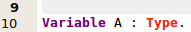
\includegraphics[scale=0.5]{../images/ide/lines.png}
                    \caption{La numérotation des lignes}
                \end{minipage}
                }
                \hfill
                \only<3->{
                \begin{minipage}[b]{0.3\linewidth}   
	                \centering
	                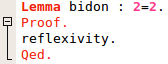
\includegraphics[scale=0.5]{../images/ide/folding.png}
	                \caption{Le ``code folding"}
                \end{minipage}
                }
                \hfill
                \only<5->{
                \begin{minipage}[b]{0.3\linewidth}   
	                \centering
	                
\includegraphics[scale=0.5]{../images/ide/redo.png}
	                \caption{Le ``Redo"}
	            \end{minipage}
	            }
            \end{figure}
        \end{frame}
            
        \begin{frame}{\coquille{} mais pas \coqide{} : Au niveau du langage}
            \begin{itemize}
                \pause
                \item La gestion de ``Ltac Debug"
                \pause
                \item Plusieurs instances de \coqtop{}
                \pause
                \item « Send / Unsend » est annulable
                \pause
                \item Affichage en version classique ou $\LaTeX$-like
            \end{itemize}
            \begin{figure}[ht]
	            \centering
	            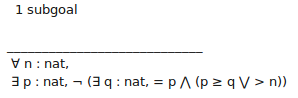
\includegraphics[scale=0.5]{../images/ide/unicode.png}
	            \caption{L'affichage $\LaTeX$-like}
            \end{figure}
        \end{frame}
        \begin{frame}{\coquille{} mais pas \coqide{} : Au niveau du langage}
            \begin{figure}[ht]
	            \centering
	            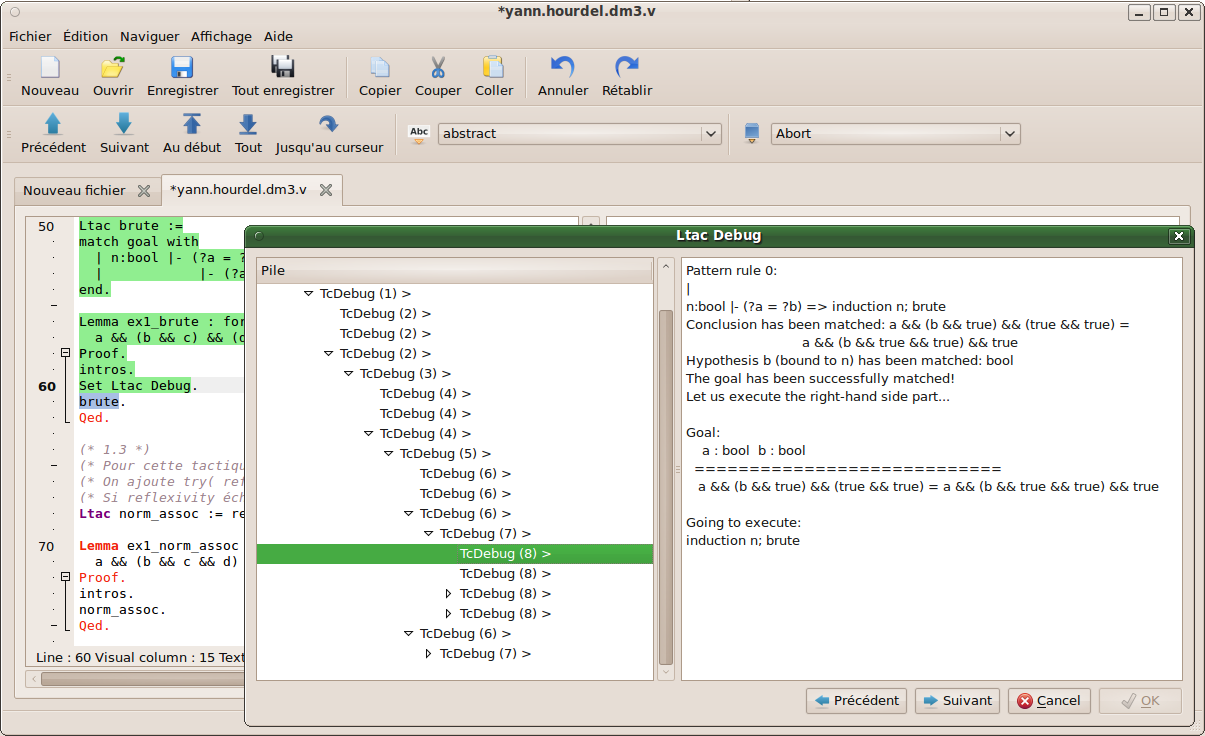
\includegraphics[scale=0.2]{../images/ide/ltacdebug.png}
	            \caption{Le mode Ltac Debug}
            \end{figure}
        \end{frame}
            
    \subsubsection{Ce que \coqide{} fait et que \coquille{} ne fait pas (encore)}
    
        \begin{frame}{Ce que \coqide{} fait et que \coquille{} ne fait pas (encore)}
            \begin{block}{Au niveau du code}
                \begin{itemize}
                    \item Lister les actions disponibles par click droit sur une hypothèse ou un but.
                \end{itemize}
            \end{block}
            \pause
            \begin{block}{Au niveau du langage}
                \begin{itemize}
                    \item Le Proof Wizard.
                    \item La gestions de la compilation et des exportations : \coqide{} permet de compiler / exporte un fichier sans passer par un terminal
                \end{itemize}
            \end{block}
        \end{frame}

    \subsubsection{Ce que ni l'un ni l'autre ne font bien}

        \begin{frame}{Ce que ni l'un ni l'autre ne font bien}
            \begin{block}{Au niveau du code}
                \begin{itemize}
                    \item L'auto-complétion
                \end{itemize}
            \end{block}
            \pause
            \begin{block}{Au niveau du langage}
                \begin{itemize}
                    \item La gestion de l'aide
                    \item La gestion des « \coqcode{Write State} / \coqcode{Restore State} ».
                \end{itemize}
            \end{block}
        \end{frame}

\subsection{Les objectifs}

    \begin{frame}{Objectifs}
        Continuer le projet si l'INRIA finit de développer une interface de dialogue avec \coq{} utilisable.

        Distribuer l'IDE de \coquille{} dans la communauté \coq{} avec un petit manuel d'utilisation.
        Un manuel programmeur basique est déjà mis à disposition.
    \end{frame}
